\documentclass[10pt]{article}
\usepackage{amsmath}
\usepackage{amsfonts}
\usepackage{amssymb}
\usepackage{graphicx}
\usepackage{hyperref}
\usepackage{url}


\begin{document}

\begin{titlepage}
   \begin{center}
       
       \huge
       \textbf{Firmware Block Implementation for the Proto-DUNE II Hit Finding Architecture with the HLS Tool}
       \vspace{0.6cm}
       
       \Large
       \textbf{Project report by J. Horswill}
       
       \vspace{0.5cm}
       
       \large 
       Supervised by K. Manolopoulos
            
       \vspace{0.5cm}
       
       \large
       Department of Physics and Astronomy\\
       University of Southampton\\
       United Kingdom\\
       \vspace{0.5cm}
       \today
       \vspace{0.5cm}
            
   \end{center}

\begin{abstract}

	The Deep Underground Neutrino Experiment (DUNE) is a large-scale international particle physics project based in North America. It will consist of two underground neutrino detectors placed within the path of an intense neutrino beam fired from Fermilab. The far detector will be 1300 kilometres from the source, in the Sanford Underground Research Facility (SURF). Objectives of the experiment include the study of certain properties of charge-parity violation (CPV) in the lepton sector, as well as the analysis of proton decay, and the investigation into black hole formation through supernova neutrino detection\cite{deep_underground_neutrino_experiment_2020}. This report focusses on the hit finder architecture of the `Trigger Primitive Generation' (TPG) cores within the front-end electronics of ProtoDUNE II. The project objective was to replace the existing firmware algorithms written for the detector's `Field-Programmable Gate Array' (FPGA) boards with designs synthesised via Xilinx's Vivado `High Level Synthesis' (HLS) software. C++ code was used to implement the desired behaviour. This enabled a comparison of the performance and utilization reports of the new designs and those written manually in a Hardware Development Language (VHDL). HLS has the potential to make firmware design more accessible to a wider range of scientists. This could lead to an increased pace in both the development of FPGA-based detector algorithms and the acquisition of important data.
\end{abstract}

\end{titlepage}



%	The Deep Underground Neutrino Experiment (DUNE) is a large-scale international particle physics project based in North America. It will consist of two underground neutrino detectors placed within the path of an intense neutrino beam fired from Fermilab, the furthest of which will be 1300 kilometres from the source, in the Sanford Underground Research Facility (SURF). Objectives of the experiment include the study of certain properties of leptonic CP violation, as well as the analysis of proton decay, and the investigation into black hole formation through supernova neutrino detection\cite{deep_underground_neutrino_experiment_2020}. This report focusses on the `Trigger Primitive Generation' (TPG) cores within the front-end electronics of the detectors. More specifically, the report discusses the hit finder architecture that processes optical data. This data is generated from argon scintillation within the `Time Projection Chambers' (TPCs), as a result of neutrino-nucleon interactions. The project objective was to replace the existing firmware algorithms written for the detector's `Field-Programmable Gate Array' (FPGA) boards, with designs synthesised via Xilinx's Vivado `High Level Synthesis' (HLS) software. C++ code was used to implement the desired behaviour. One of the end goals was to allow the comparison of the new design's performance and resource utilization to those written from scratch in the VHSIC Hardware Development Language (VHDL). HLS has the potential to make firmware design more accessible to a wider range of scientists. This could lead to more people contributing to improving the capability and performance of particle physics detectors and consequently acquiring groundbreaking data at a faster pace.

\newpage
\tableofcontents

\section{Introduction}

\subsection{DUNE Experiment Goals and Context}
The DUNE experiment is an amalgamation of many neutrino-physics communities, centred around an opportunity provided by the large investment of the U.S. Department of Energy. This will contribute to a large expansion of the underground experimental architecture of the SURF facility, as well as a megawatt neutrino-beam facility 1300km across North America at Fermilab. This investigation will be groundbreaking for several areas of physics, including neutrino oscillation studies, searches for proton decay, and for neutrino-based astrophysics i.e. black hole and supernova burst phenomena.

Analysing the properties of neutrinos has led to evidence for physics beyond the Standard Model (SM). Oscillations of neutrino flavour is a well established concept, from which several conclusions can be made. The first is the fact that neutrinos have mass, although unexpectedly small; the sum of the three neutrino mass eigenstates must be less than one million of an electron mass eigenstate \cite{Mertens_2016, cooper2016masses}. The origin of these small neutrino masses and their oscillations is still not confirmed however, and is up for discussion. Finding the explanation will require access to more precision and detail in the available experimental data. DUNE exists to carry out an investigation of neutrino oscillations to test lepton sector CP violation (LCPV) as well as the ordering of the neutrino masses and the three-neutrino paradigm\footnote{The quantum mechanical mixing of the three neutrino mass eigenstates producing the three known neutrino flavour states \cite{acciarri2016longbaseline}}.

CPV is well established in Quantum Chromodynamics (QCD), allowed by the complex-natured Cabibbo-Kobayashi-Mashawa (CKM) matrix\footnote{Used to contain the information on the strength of the flavour-changing weak interaction \cite{kobayashi1973cp}.}\cite{kobayashi1973cp}. Therefore one would expect to discover an entirely analagous mechanism to arise in the lepton sector of the standard model (SM), leading to LCPV. One of the collaboration's goals is to determine the rates at which neutrino CP violation occurs within the lepton sector. Another hypothesis proposes that there is a connection between low-energy neutrino physics and leptogenesis \cite{Di_Bari_2012}, which could provide insight into the scenario that led to the baryon asymmetry of the universe. These questions can only be answered by constructing suitable detector equipment; the next section will explore the features of ProtoDUNE's detector's front-end electronics and Data Acquisition (DAQ) system. This will feed into the following section that discusses the HLS firmware blocks that could instruct the front-end FPGA-based data processors.

\subsection{The Importance of Neutrinos in the Standard Model}

\subsection{ProtoDUNE DAQ System}\label{section:overview}

DAQ architecture can be split into two parts: the front-end and the back-end. The front-end is comprised of circuitry that acquires the data stream from readout-electronics inside the TPC detector, so that it can process and deliver the stream to the back-end: an offline storing, event-reconstruction computation farm. The focus of this report will be on the front-end, including the detection modules and the interface to the detector electronics.

There are several main factors that influence the design of the DUNE DAQ system. One of which is the hardware and maintenance cost per input channel, which is related to the technology life-cycle of each component. This contributes to the need for long-lasting essential parts such as the Xilinx FPGAs and network components. DUNE is set to run for approximately 20 years; the reliability and maintenance of the detector components is more important when compared to other large-scale projects. The power consumption of the detector modules also requires consideration due to cooling contingencies and the variance in running costs.  Modularity of the hardware and firmware blocks is emphasised, so that one change in a sub-module would not affect the rest. This emphasis on customisability carries over to the HLS design process. If the design tools are more abstract and are rooted in commonly used languages such as C++, this will appeal to the vast majority of users (physicists) \cite{abi_barr_martin-albo_azfar_2017}. For more detail on this matter see section \ref{HLS_section}. With these objectives in mind, R\&D and fast firmware modifications can be a quick and efficient process. 

\subsubsection{Single and Dual Phase LAr TPCs}

The use of Time Projection Chamber modules of Liquid Argon (LAr TPCs) is a matured and popular technique used by several short-baseline\footnote{The baseline refers to the scale of the beam travel distance. DUNE is `long baseline' as the detector is positioned across the continent from the beam source.} neutrino experiments. They are popular for several reasons:

\begin{itemize}
	\item Argon is a noble element of vanishing electronegativity, which means that electrons produced by ionizing radiation will not be absorbed as they drift towards the detector.
	\item  Liquid Argon is inexpensive yet very dense, increasing the likelihood of a particle interacting by 1000 times when compared to Nygren's TPC design \cite{rubbia1977liquid}. This is important because the cross section for neutrino-nucleon interactions is very small.
	\item A neutrino-nucleon interaction causes the Argon to scintillate; a secondary energetic charged particle is generated and travels through the liquid, which causes the release of scintillation photons, the number of which is proportional to the energy deposited by the passing particle \cite{adams2018rejecting}. This contributes to the reconstruction of the event. 
	
\end{itemize}

\begin{figure}
	\centering
	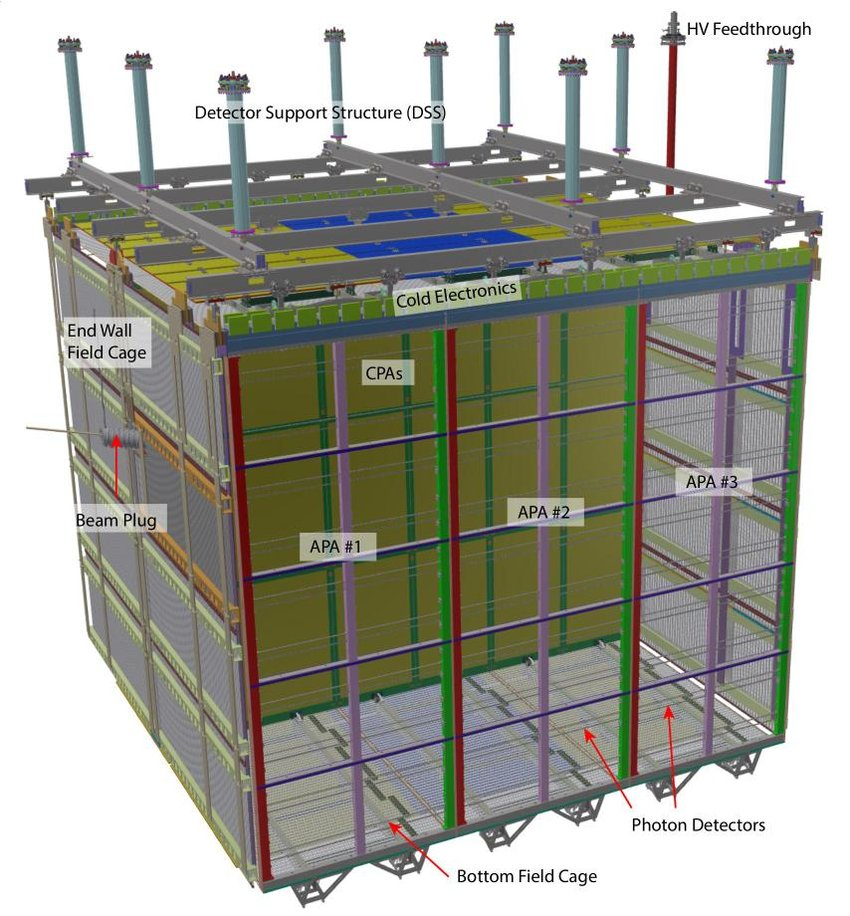
\includegraphics[width=0.7\linewidth]{figures/The-major-components-of-the-ProtoDUNE-SP-TPC}
	\caption[ProtoDUNE-SP]{Diagram of the ProtoDUNE single-phase LAr TPC module. This contains two drift volumes, separated by a central cathode plane that is flanked by two anode planes, connected to a field cage that surrounds the entire module. Each anode plane is made of three Anode Plane Assemblies (APAs). These connect and send data to the front-end electronics being discussed in this report \cite{dune_sp_collab}.}
	\label{fig:the-major-components-of-the-protodune-sp-tpc}
\end{figure}


 There exists both single and dual-phase versions of these LAr TPC modules. Inside single-phase liquid argon detectors, such as the structure featured in figure \ref{fig:the-major-components-of-the-protodune-sp-tpc}, the interactions are readout by wires immersed in the liquid and do not require the amplification of the ionized electron charge. The charge is localised using alternative induction and collection wire planes with different orientations. This was tested by ProtonDune-SP at CERN \cite{dune_sp_collab}.
 
 The dual phase detectors rely on the amplification of ionisation charges in the ultra-pure cold-argon vapour layer above the liquid. In dual-phase LAr TPCs, ionisation charges produced by neutrino interactions drift vertically towards the liquid-vapour boundary where they are extracted into the gas phase, amplified by components named Large Electron Multipliers (LEMs), and collected by segmented anodes. Five photo-multiplier tubes are mounted underneath the TPC drift cage. They detect the Argon (prompt S1) scintillation photons formed from interactions with passing charged particles, as well as the (proportional S2) secondary scintillation light from the electroluminescence of the electrons extracted in the argon vapour. S1 is at least several orders of magnitude higher in detection amplitude than S2 in a tested TPC \cite{aimard20184}.
 
 The 10 kilo-tonne dual-phase liquid argon TPC is one of the main detector options considered for DUNE. LAr TPC's offer unprecedented 3D imaging capabilities and the functionality of a homogeneous calorimeter. High-resolution imaging is the key to efficient background noise rejection.

\subsection{FELIX}

The LAr TPC modules used in the ProtoDUNE II design contain 150 APAs, each containing 2560 wires. There are 10 fibres/data streams in the APA, filled with 256 wires per fibre. The Front End LInk eXchange (FELIX) system is used to receive the data from the APAs, and was first developed within the ATLAS collaboration. Within this system contains the focus of this project: the TPG core, discussed in section \ref{tpgcoresec}. FELIX is a PC-based networking gateway with the FPGA mounted on PCIe\footnote{High speed connection ports used in motherboards to connect GPUs, SSD's, wifi chips and more.} Gen3 cards \cite{borga2019felix}. In ProtoDUNE II, FELIX interfaces with and manipulates the data from the APA, during which time it is fed through the TPG core within the Hit-Finder (HF) processor.

The readout window per neutrino event is between 3-5.5 ms for a 2.25 ms drift time. The FELIX architecture that handles this influx of events consists of 10 MGT modules. The function of an MGT is to process the APA data stream into computational bits, which are then fed into 10 HF processors, as seen in figure \ref{fig:fearch}. The hits are produced by processing the incoming ADC (Analog-to-Digital Converted) samples in parallel. The MGT output enters the HFs via the data router, which receives multiple-channel, single clock-tick packets. The packets initially exist in a format containing a given sample wave for all channels, and when processed by the data router are converted into a format subsisting of all the samples for a given channel i.e. multiple clock ticks of data. The formatted output is then transferred into 10 sets of 4 TPG block processors; one set for each MGT output. The processor outputs are multiplexed\footnote{Combined into a singular signal output.} by the arbitrator into the Central Router (CR) interface \cite{abi_barr_martin-albo_azfar_2017, adams2020protodune} as seen in figure \ref{fig:hfprocessor}.

\begin{figure}[h]
	\centering
	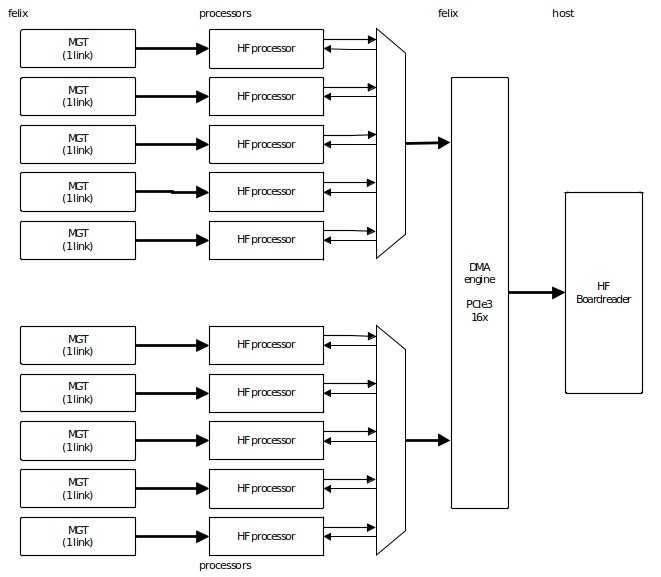
\includegraphics[width=0.7\linewidth]{figures/FE_arch}
	\caption{Overview of the Felix architecture in ProtoDUNE \cite{manolopoulos_2020}}
	\label{fig:fearch}
\end{figure}

\begin{figure}
	\centering
	\makebox[\textwidth][c]{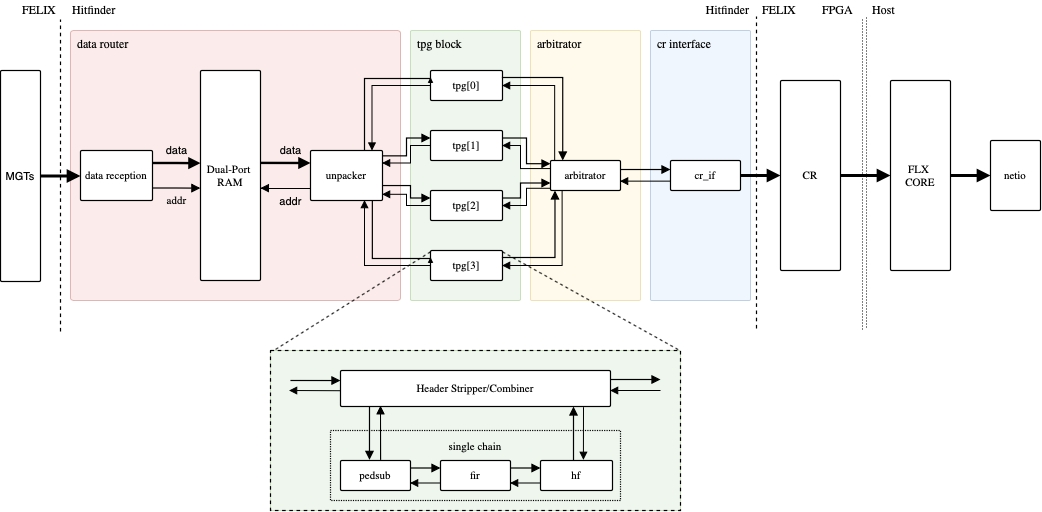
\includegraphics[width=1.6\linewidth]{figures/HF_processor}}
	\caption{Hit Finder Firmware Architecture \cite{manolopoulos_2020}.}
	\label{fig:hfprocessor}
\end{figure}

\subsection{The TPG Core}\label{tpgcoresec}

Each TPG unit processes the data from 64 APA wires, and so there are 4 units for each core\footnote{$4\times 64 = 256$, the number of wires in a fiber; ten fibers summed over ten MGTs accounts for all wires within the APA (2560).}.
The TPG data consists of a header and a payload. The header determines the source wire, the time stamp, and the origin of the data. The payload is 64 bits of ADC sample data for hit finding. There is an AXI4-stream protocol for the unpacking and reordering of data in the TPG block, featuring 6 general signals for various instructions in each component:


	\begin{enumerate}
		\item \texttt{tvalid} denotes if the bus data is valid for processing.
		\item \texttt{tkeep} goes high when the incoming data should be processed.
		\item \texttt{tuser} is a flag that denotes the end of a packet frame.
		\item \texttt{tlast} indicates the end of a packet.
		\item \texttt{tready} is used to apply back-pressure if the processing units ahead cannot process the data fast enough (all throughput is frozen).
		\item \texttt{treset} goes high when the entire process must be reset and restarted, sometimes used when an error in the FELIX interface occurs.
	\end{enumerate}

Within the TPG core is a mechanism that strips the packet header: the Header Stripper/Combiner (HSC), featured in figure \ref{fig:hsc}. The header is sent to the output of the block. Meanwhile, the remaining 64 ADC samples and their associated AXI4-S signals are processed by the PedSub (pedestal subtraction), FIR (finite impulse response), and HF sub-blocks in the chain. The data router is then signalled to send the next packet forward for input.

The objective of this project is to redesign the firmware algorithms for the TPG sub-blocks in Xilinx's Vivado HLS software suite. This is to acquire a comparison of the performance and resource usage of the HLS design with the existing firmware written by VHDL engineers. Section \ref{HLS_section} goes into more detail on this matter.

\begin{figure}
	\centering
	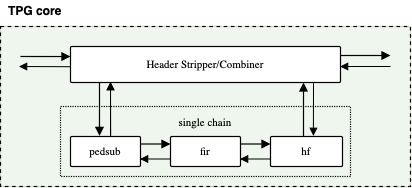
\includegraphics[width=0.7\linewidth]{figures/HSC}
	\caption{Focus on the HSC and the sub-block chain \cite{manolopoulos_2020}.}
	\label{fig:hsc}
\end{figure}

\section{HLS}\label{HLS_section}

\subsection{Background}
High-level synthesis (HLS) is an automated design process that interprets an algorithmic description of a desired behavior and creates digital hardware that implements that behavior. It was initially designed to increase the levels of abstraction for design methodologies, forced by the growing capabilities of silicon technology and the increasing complexity of their applications. Beginning in the 1950s, assembly languages were introduced and gradually evolved to high level languages with improved compilation techniques, obeying the intuitive rules of grammar, syntax and semantics. Gate-level simulations appeared in the 1970s, and in the 1980s progress led to Hardware Description Languages (HDLs). A HDL is a programming language that describes the structure and behaviour of electronic circuits, and more commonly digital logic circuits \cite{coussy2009introduction}. HDLs look like programming languages such as C, but the main difference is that they include the notion of clock timing. The most commonly-used languages are Verilog and VHDL, the latter of which is used in the DUNE firmware framework. HLS allows for a connection between software languages and hardware implementation. In the case of section \ref{pedsubalg} this is achieved via VHDL firmware. 

Synthesis begins with a high-level specification of the problem, where behavior is generally decoupled from low-level circuit mechanics such as clock-level timing. Early HLS explored a variety of input specification languages, although recent research and commercial applications generally accept synthesizable subsets of ANSI C, C++, SystemC and MATLAB. C++ was used to design the algorithms featured in section \ref{pedsubalg}. This input source code is analysed, architecturally constrained, and scheduled to transcompile into a register-transfer level (RTL) design in a chosen HDL, which is in turn commonly synthesized to the gate level by the use of a logic synthesis tool \cite{vivado_design_suite_user_guide_2018}.

RTL is a design abstraction which models a synchronous digital circuit in terms of the signal flow between registers and the logic operations being performed on said signals \cite{vahid2010digital}. Hardware registers are circuits composed of flip flops: a sub-circuit that has two stable states used to store state information. They are a basic storage element in sequential logic, possessing the ability to read or write multiple bits at a time and use an address to select a particular register, used as an interface between the software and the computer peripherals \cite{bose1996hardware}. RTL allows for circuitry simulation and digital analysis, and is used in HDLs to create high-level representations of a circuit, from which lower-level representations and ultimately actual wiring can be derived. RTL clock cycle data is given in Vivado HLS performance estimate data, as it can read how long a certain block, loop or function in the code took to complete; this is called the latency. Latency is a crucially important concept in RTL design, as it can make the difference between a system struggling with logic timing issues and a synchronised circuit. Before the firmware block in question can be discussed, the design flow within Xilinx's Vivado HLS development software will be explained to provide context for the generation of the algorithm.


\subsection{Vivado HLS Design Flow}
\label{section:HLS_DF}

The design flow when approaching the synthesis of a C algorithm is as follows:


\begin{enumerate}
	\item Compile, simulate, and debug the C algorithm.
	
	This involves validating that the C program correctly implements the required processes. In order for this to occur, there must be a test bench written in C that includes the top-level function called within a simulation script, tasked with recreating the conditions of the implemented firmware, hosted within \texttt{main()}. This typically takes more time to design than the function to be synthesized.
	
	\item Synthesize the C algorithm into an RTL implementation, optionally employing user optimization directives.
	
	This allocates hardware resources such as BRAMS, buses, look up tables (LUTs), digital signal processors (DSPs) and registers. Each operation is scheduled to a certain clock cycle and bound to a functional unit within the board. Variables are bound to storage elements, and the RTL architecture is eventually generated\cite{vahid2010digital}. See section \ref{direct} for more information on directives.
	
	\item Generate comprehensive reports and analyze the design.
	
	After C synthesis, output files are stored in a directory which contains folders for each RTL output format, and a report folder. The report folder contains files reporting on the performance and design corresponding to the top-level function and each individual subfunction. The analysis tab allows for cycle-by-cycle insight into the timing of logic operations and the FPGA resource consumption that they require. This is the best opportunity to analyse the effect of applied function directives and \texttt{pragma}\footnote{Pragmas are directives that are stored within the source code, rather than in an external \texttt{tcl} file} commands.
	
	\item Verify the RTL implementation using a pushbutton flow.
	
	 This is a post-synthesis validation process that compares the synthesised RTL and C programs to see if they generate the same output; this is called C/RTL co-simulation.
	
	\item Package the RTL implementation into a selection of IP formats.
	
	This generates the verified VHDL script that can be synthesized in the Vivado project manager into an implementable design. Before this can occur, a wrapper is written to connect the IP block's I/O ports to the previous and following blocks, ensuring signals are being properly read and written. This is especially important for the AXI4 stream protocol discussed in section \ref{tpgcoresec}, as all boolean signals must enter and leave the block for the AXI4 interface to be able to validate and manage the incoming and outgoing data samples. This can be tested in Questasim\footnote{Software dedicated to simulating HDLs. This is typically used in collaboration with the Vivado project manager environment, where full VHDL block chains can be synthesized and implemented within the FPGA.} to provide a waveform analysis of every port and internal register involved. This is an important verification step in the design process, as the performance of an algorithm within the HLS environment can be vastly different to a VHDL simulation \cite{vivado_design_suite_user_guide_2018}.
\end{enumerate}

When writing HLS source code, there is punishment for using modern modules and storage entities; a simplified, classical style is most easily synthesized. An example of this is that storage arrays must have pre-allocated memory, with a determined number of elements at compile time (ruling out C++ vectors).

The performance of the logic operations come into question when constrained by a certain latency in order for the block to operate as required. The clock period must simultaneously stay below $1/f_{target}$, which in the case of the the TPG core, the target frequency $f_{target} = 250$ MHz, meaning the clock duration must stay below 4ns. However, it must tick for long enough so that the block operations can occur within the desired latency. Performance comes at a trade to resource cost, as pipelining (parallelizing and rearranging operation initialisation to decrease the latency and input interval) employs more FPGA elements, which are a finite resource. One way to reduce this cost is to assign accurate bit-widths to variables. Using standard C data types for hardware design results in unnecessary resource usage. Operations can use more LUTs and registers than needed for the required accuracy, causing delays that may exceed a given clock cycle, increasing the overall latency. Smaller bit widths (e.g using 17 bit data types for 17 bit multiplication rather than the standard C 32 bit data type) result in hardware operators which are smaller and faster. More logic can then fit in the FPGA which can operate at a higher clock frequency. The next section will discuss the management of performance and area when choosing HLS design guidances.

\subsubsection{Optimisations and Analysis}\label{direct}

Directives act as a low-level guidance for the HLS tool, influencing the types of hardware used and the methods of implementing the source code operations. An example of this is the partitioning of an array into registers, allowing for faster data access at the cost of increased resources \cite{lo2016model}. Different optimization directives can be applied before C synthesis; one of the most crucial is the \texttt{pipeline} directive which instructs a code task to execute non-sequentially, allowing the next execution of a task to begin before the current one finishes. Alongside this, the user can employ a specification for the minimum or maximum latency for a task, loop or for the whole function (one of the reasons for this is to match the FPGA clock frequency). Not only can performance be adjusted by directives, but the HLS tool can also specify a limit to the resources used by the block, allowing for a balance between speed and area usage. Additionally, more customisation opportunities arise from the ability to select a block's I/O protocol to make sure the final design can be connected to other hardware blocks with the same framework.

There are several viable ways to achieve an optimal directive configuration for the purposes of the user, but the best way to gauge the effect of adding directives in the Vivado HLS tool is by analysing the cycle-by-cycle display of operations within the synthesis reports. One can analyse a number of aspects surrounding the performance estimates of the block, perhaps the most important of which is clock timing. This is the fastest achievable clock frequency before the block ceases to function. This must meet the target to synchronise with the surrounding firmware blocks. Secondly, the block latency and initiation interval\footnote{The number of clock cycles before new inputs are processed.} (II) must be reviewed, since the internal operations of the block must have enough time to complete before the next input is processed. Without any pipeline directives, the latency defaults to one clock cycle less than the II so that this can be achieved. Finally, the utilization estimates are key to making the trade-off between latency and FPGA area, be it LUTs, FFs, DSP48s or BRAMs. Limited budget and gate area means that unlimited resource usage is not an option, therefore this must be tracked.

Now that a sufficient introduction into the design process has been given, the next section will explore the key work outlined in this report: the HLS firmware algorithm employed by the first sub block in the HSC (discussed in section \ref{tpgcoresec}).

\section{Development and Findings}

\subsection{Pedestal Subtraction Algorithm}\label{pedsubalg}

The pedestal subtraction algorithm was the first mechanism to be redesigned in HLS. It removes background noise from the incoming event data, so that the following FIR and HF blocks are dealing with isolated optical signals from the neutrino events occurring within the detector. It is employed by the first sub-block in the TPG core, \texttt{pedsub}, which is fed by 64 sample words\footnote{Known as a data packet, each sample contains an input ADC value and the associated AXI4 signals.} from the Header-Stripper/Combiner shown in figure \ref{fig:hsc}.  Before the performance and resource utilization can be compared to the original design, it is necessary to demonstrate the algorithm's mechanisms.

\subsubsection{Algorithm Operations}

The packet begins with 70 sample words, however the first 6 16b words are stripped from the incoming samples and sent to the \texttt{pedsub} block. There are three important variables used to achieve the reduction of background noise: the pedestal (or median), the accumulator, and the incoming ADC sample. The pedestal acts as the average background signal for a given channel, used to subtract from the data samples to produce the `true' values. The pedestal and accumulator are adjustable values that must be set to an estimate before any samples have entered the block. When the pedestal is greater than the incoming ADC value, the accumulator is decreased by one, and if the opposite is true, the accumulator is increased by one. When the accumulator reaches a limit of $\pm 10$, the pedestal is increased by one or decreased by one respectively, and the accumulator is reset. See figure \ref{fig:pedsubalg} for an illustration of how the algorithm manages signal noise.

Connected to (or implemented within) this block is a State Save/Restore (SSR) mechanism, which is used to save these adjustable variables at the end of a packet. The mechanism is implemented via a VHDL source file connected to the \texttt{pedsub} wrapper, that receives and feeds values to the pedestal subtraction block. This allows for a variable restoration every time a packet enters a pre-processed channel, allowing for an array of algorithm-tuned median and accumulator values to be used for the remainder of the detector run time. Therefore once \texttt{tlast} goes high, the final pedestal and accumulator values for the current channel are saved and those saved from the next channel are retrieved from the SSR. Every 64 packets, a saved value is again restored for the next packet entering the same channel. This is because packets are processed for each channel sequentially, beginning from 0 and reaching channel 63. This means that once the \texttt{pedsub} block has run for every channel, there will be a better background noise estimate and therefore more accurate ADC output data.  Eventually, with a large enough flux of packets, one would obtain an optimal pedestal value appropriate for the background noise of each input channel.

\begin{figure}
	\centering
	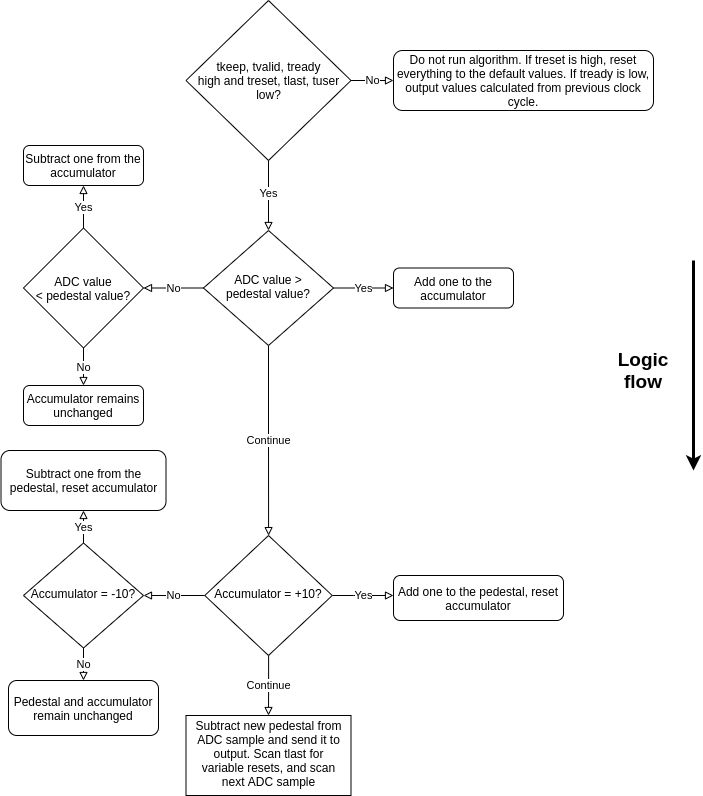
\includegraphics[width=.8\linewidth]{figures/PedSub_Alg}
	\caption[Pedestal subtraction algorithm]{Flow chart detailing the logic flow of the pedestal subtraction algorithm, demonstrating the adjustment of the pedestal and accumulator values, as well as the occurrence of the subtraction from the ADC value.}
	\label{fig:pedsubalg}
\end{figure}


\subsubsection{Redesign of Pedestal Subtraction with External SSR}

The development and debugging of the \texttt{pedsub\_HLS} block led to a number of insights for future use of high-level synthesis when designing detector firmware. The first thing to note is that when developing an algorithm, it is advisable to start with a simplified version of the target function. This is because complex functions are especially prone to invalid signals and incomplete output, which can be difficult to debug when trying to trace back the unfamiliar proxy signals in machine-written VHDL code. One could argue that it is better to fix output issues within the HLS environment rather than try to treat `symptoms' of the problem by editing the IP block file. One of the best approaches would be to slowly add layers of complexity, and each time an addition is made, test the functionality in Questasim and observe successful synthesis in the Vivado project manager before adding more.

Part of the design process involves ensuring that for every input port dealing with the incoming sample word, there must be an output port. This allows the continuation of each signal to the surrounding blocks. One must also include contingencies in the wrapper for the disparity between the IP block and wrapper port's bits widths, as well as the timing of signals, such as with the internal variable restoration when \texttt{tlast} goes high. This links into the inclusion of static variables that save internal values between function calls.

The Vivado HLS synthesis tool recognises a static variable in the same way a C++ compiler would, generating a static storage area for that value. An example of their use in the pedestal subtraction algorithm is the storage of a clock cycle counter that starts when the \texttt{tlast} signal output goes high. This static variable is saved between multiple function calls until it reaches three cycles. When this happens, the statically-stored pedestal and accumulator values are restored to their values for the next channel. Static variables are a crucial tool when a self-sufficient block is required and externalised I/O management blocks are inconvenient. However, one main issue is faced in the long-term storage of the pedestal and accumulator: static variables are wiped between incoming packets. In the Questasim simulations this occurs five clock cycles after the \texttt{tvalid} signal goes high. A separate SSR storage array mechanism must be developed for restoring values for a given channel in the long term. HLS is inconvenient when developing an SSR mechanism in this case; the block being called every clock cycle means that new declarations are reset very frequently, unless they are static. Further investigation needs to be made into the optimal approach.

The automatic static variable wipe happens too late; the restoration of values 5 clock cycles after \texttt{tvalid} goes high means that the first 5 subtractions occur using the previous packet's pedestal, which leads to 5 invalid results for the next channel. A manual restoration of the internal values must occur before \texttt{tvalid} goes high for the next packet. However, this restoration must be after the previous packet's \texttt{tlast} output goes high; the \texttt{tlast} input is not used as this would still truncate the last value. This restoration window is prioritised in order to avoid invalidating the previous packet's ADC output values. It was found that restoring 3 clock cycles after the tlast output goes high allows for the restoration of the pedestal and accumulator to occur from the existing SSR mechanism.

One additional timing concern is ensuring that the outputs are transmitted at the same pace that the inputs are received, which can be achieved with the \texttt{pipeline} directive mentioned in section \ref{direct}. 



\subsubsection{Performance and Resource Utilization Comparison}

\begin{figure}
	\centering
	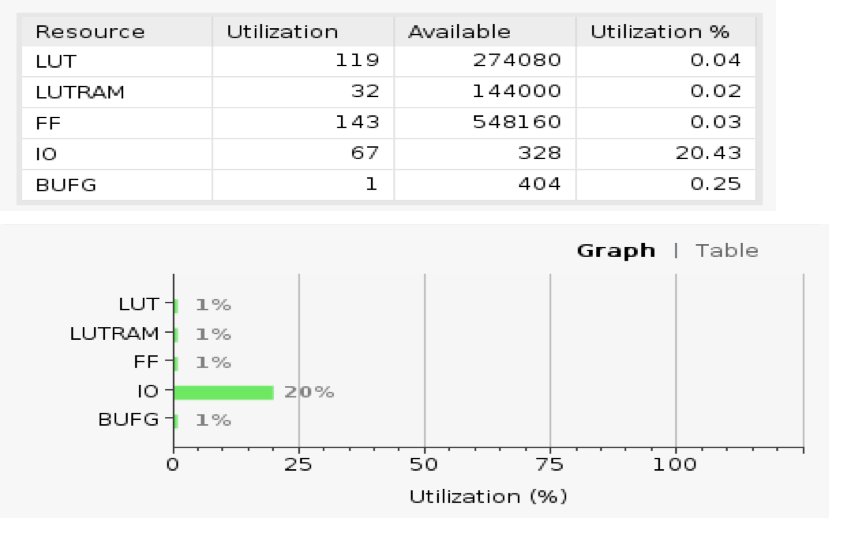
\includegraphics[width=0.7\linewidth]{figures/pedsub_block_stats}
	\caption[Original algorithm resource usage]{The resource utilisation for the original pedestal subtraction block, including the exact figures above and percentage utilization below, taken from a Vivado Project Manager post-implementation report summary.}
	\label{fig:pedsubblockstats}
\end{figure}

\begin{figure}
	\centering
	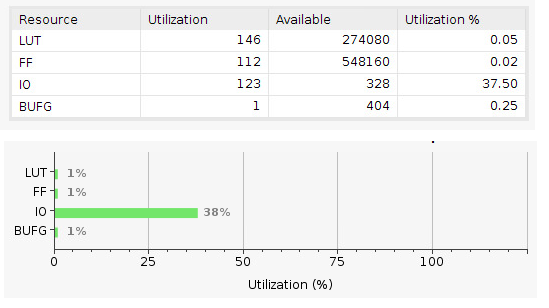
\includegraphics[width=0.7\linewidth]{figures/HLS_block_stats}
	\caption[HLS algorithm resource usage]{The resource utilization of the new HLS block, including exact figures above and percentage utilizations below, sourced from the Vivado Project Manager post-implementation report summary.}
	\label{fig:hlsblockstats}
\end{figure}

The HLS block was forced to perform at a max latency of one clock cycle with an II equal to the latency, meaning the outputs arrive one cycle after the inputs and the inputs are accepted every clock cycle. This can be compared to the performance of the existing algorithm which has a latency of two and an II of one. The synthesis report shows the block has a clock cycle of 3.6$\pm 0.5$ nanoseconds, and an RTL co-simulation confirmed the block satisfies the target frequency of 250 MHz and a confirmed latency of one clock cycle. The HLS block outputs the same values as the previous design, with a 1 clock cycle delay due to the difference in latency. This was verified by a ModelSim simulation comparison between the blocks, and several model software output files.

When comparing resource utilisation, the most important resources to compare are LUTs, LUTRAM and FFs. From figures \ref{fig:pedsubblockstats} and \ref{fig:hlsblockstats} we can deduce that the new design requires $0.01\%$ more LUT usage, less (almost negligible) FF usage, but a substantial difference in I/O usage. The reason for the increase in LUT usage from the HLS block is the directive forcing performance at a one clock cycle latency, which could be changed to reduce resource usage even further. The I/O disparity is linked to the increased number of ports required in the HLS design for this instance.

The original block includes the SSR within the utilization estimates, which is why the corresponding table contains LUTRAM usage. The HLS block used an external SSR mechanism not included within the estimates, hence no LUTRAM is featured.

\subsubsection{Pedestal Subtraction with Implemented SSR}

\subsubsection{BRAM Utilisation for the SSR Mechanism}

One read and/or write per clock, this is ok though for accumulator and pedestal restore.

\subsubsection{Performance and Resource Utilization Comparison}

\subsection{Finite Impulse Response Filter}

\subsubsection{Algorithm Operations}

\subsubsection{AXI4 Stream Protocol Directive Method for Back Pressure Behaviour}

Include stuff about struct inputs and side channels also. tuser bug? Talk about ap\_rst\_n solution to axis directives.

\subsubsection{Redesign of FIR with External SSR}

\subsubsection{Timing and Accommodating the Tap Restoration}

\subsubsection{Performance and Resource Utilization Comparison}

\subsubsection{FIR with Implemented SSR}

One read and/or write per clock, talk about 32/32 split of restore and save. Taps were partitioned into registers and accessed all at once, but not by multiple loops at the same time (dependency). Completely partitioned arrays into registers can do almost anything you want, compared the limited access of BRAMs.

In this way, talk about the dependency workaround (for fir\_HLS\_SSR) of using two sets of taps for register shift and sum, as well as the SSR\_temp registers for the SSR mechanism. 

\subsubsection{Optimising for Back Pressure Functionality}

\subsubsection{Performance and Resource Utilization Comparison}

\section{Design Processs Conclusions}

\subsection{Simulation using Questasim}

Talk about partially-pipelined designs (II average = 1, max = 2) often not being compatible with the questasim simulation. Lots of other problems encountered. Waveform debug and outputFile.txt worth mentioning.

\subsection{Timeline analysis}

Analysing time duration of certain processes in the analysis tab?

\section{Future of High Level Synthesis and the DUNE Experiment}

\bibliographystyle{ieeetr}
\bibliography{dpn.bib}


\end{document}